% $Id: polyarith.tex,v 1.1 1992/05/10 19:43:45 rz Exp rz $
\chapter{Bounds on Polynomials}
\label{PBounds:Chap}


The more sophisticated polynomial algorithms discussed in the following 
chapters require
estimates on the size of the coefficients of factors of a polynomial.
The most natural of these results give bounds on the size of linear
factors of univariate polynomials, \ie, bounds on the size of zeroes
of univariate polynomials.  These bounds are very useful when
computing the polynomial zeroes numerically.  The linear factor
estimates can be extended to give bounds on the size of larger degree
factors.  These estimates are
used in calculations of the {\sc gcd}'s and factorizations of polynomials
over the integers.

\sectref{PB:Heights:Sec} makes precise how to estimate the size of a
polynomial, taking into account the size of the coefficients.  These
different ways of measuring the size divide into two different
classes, those that give equal weight to all of the coefficients and
those that give different weights to coefficients of terms of
differing degrees.  In \sectref{Uniform:Bounds:Sec} bounds
on the size of the coefficients based on unweighted size
measures are derived.  \sectref{Weighted:Bounds:Sec} presents bounds that
make use of weighted coefficients size measures.  

Bounds sharper than those of \sectref{Uniform:Bounds:Sec} can be
derived for the special case of linear factors, \ie, for zeroes of a
polynomial.  These results are given in \sectref{PB:RootSize:Sec}.
Finally, in \sectref{PB:RootSeparate:Sec} we give lower bounds on
distance between two roots of a polynomial, \ie, $|\alpha_i - \alpha_j|$.

\section{Heights of Polynomials}
\label{PB:Heights:Sec}

We begin by defining a few different measures on the size of the
coefficients of $P(X)$, 
\begin{equation}\label{PA:p:Def:Eq}
P(X) = p_0 X^d + \cdots + p_{d-1} X + p_d,
\end{equation}
where $p_0 \not= 0$.

We define the {\em height}\index{height, of a polynomial} of a $P(X)$ to be 
\[
\|P \|_{\infty} = 
  \max \{\left|p_{0}\right|, \left|p_{1}\right|, \ldots, \left|p_{d}\right|\}.
\]
In the notation of \chapref{Lattice:Chap} this is the $\|\,\|_{\infty}$ norm
of the vector $\langle p_{0},\ldots, p_{d}\rangle$.  Similarly, we define the
$\|\,\|_{2}$ norm of a polynomial by
\[
\|P \|_{2} = \left(\left|p_{0}\right|^{2} + \cdots +
    \left|p_{d}\right|^{2}\right)^{1/2}.
\]
In the literature, some authors use $|P|$ for $\|P\|_{2}$, while
others use $|P|$ to mean $\|P\|_{\infty}$.  The first notation is
common in the computational complexity community, while the second is
more common in diophantine analysis.  Since we feel that using $|P|$
for $\|P\|_{\infty}$ is slightly more mnemonic and is also consistent
with the notation used for norms of vectors in \chapref{Lattice:Chap}
we choose to follow the practice of the diophantine analysis community
and use $|P|$ for $\|P\|_{\infty}$ and $\|P\|$ for $\|P\|_{2}$, when
$P$ is a polynomial.  The relationship between these bounds is given
by the following proposition.

\begin{proposition}\label{PB:HeightRel:Prop}
Let $P$ be a univariate polynomial of degree $d$ over $\C$.  Then
\[
|P| \le \|P\| \le \sqrt{d+1} |P|.
\]
\end{proposition}

\begin{proof}
$|P|$ is equal to $\|P\|$ if only and if all but one of the coefficients
of $P$ are zero.  Otherwise $|P| < \|P\|$.  Let $p_{\ell}$ be the
coefficient of $P$ with the largest absolute value. Then
\[
\|P\|^2 = |p_0|^2 + |p_1|^2 + \cdots + |p_d|^2 \le (d+1) |p_{\ell}|^2.
\]
\end{proof}

When $P(X) = F(X) G(X)$, one might expect the height of $F$ to be less
than the height of $P$.  This is obviously true if $F$, $G$ and $P$
all have positive coefficients; however, it is not true in general.
The canonical example along these lines is the factorization of
$X^{n}-1$ over the rational integers.  Though it is plausible that the
coefficients of the factors of $X^{n}-1$ all be $\pm1$, in fact they
can grow rather quickly. The smallest example for which $f$ has height
greater than $1$ is $n=105$.  $X^{105}-1$ has an irreducible factor of
degree $47$ that has two terms whose coefficients are $-2$.  Even
larger coefficients can be found by factoring higher degree cyclotomic
polynomials. In fact, {\Erdos} has shown \cite{Erdos1946-ns}:
\begin{proposition} [\Erdos]
Let $A_n$ denote the absolute value of the largest coefficient in an
irreducible factor of $X^n -1$.  For infinitely many $n$
\[
A_n > e^{c (\log n)^{4/3}}
\]
for some positive coefficient $c$.  In particular we can take $n = 2
\cdot 3 \cdot 5 \cdots p_k$.
\end{proposition}

\Marginpar{Bad transition to this point.}Another useful measure of a polynomial's size is how far outside the 
unit disk its zeroes lie.  Denote the zeroes of $P(X)$ by $\alpha_1,
\ldots, \alpha_d$.  We define $M(P)$ to be
\[
M(P) = |p_0| \prod_{1\le i \le d} \max\{1, |\alpha_{i}|\},
\]
which is the product of the absolute values of the zeroes of $P(X)$ that
lie outside the unit disk.

All of the polynomial norms discussed thus far treat each of the
coefficients equally.  However, when multiplying polynomials the
``middle'' coefficients tend to get larger more quickly than the
leading and trailing coefficients, \eg{}
\[
(X+1)^5 = X^5 + 5 X^4 + 10 X^3 + 10 X^2 + 5 X +1.
\]
By the Caucy product formula \eqnref{PolyCauchyProduct:Eq},
the interior coefficients of a product are the sum of more terms than
the coefficients closer to one or the other end of the polynomial.

A norm that takes advantage of this behavior was introduced by
{\Beauzamy} \etal{} \cite{Beauzamy1990-yo}.  The {\em weighted $L_2$ norm} of
$P(X)$ is defined to be
\begin{equation} \label{PB:Beauzamy:Eq}
[P(X)]_2 = \left(\sum_{i=0}^d \binom{d}{i}^{-1} |p_i|^2\right)^{1/2}.
\end{equation}

\section{Uniform Coefficient Bounds}
\label{Uniform:Bounds:Sec}

The goal of this section is to establish unweighted bounds on the size
of the coefficients in a factor of a polynomial.  The most natural
norm to use for this purpose is the height of the polynomial, $|P|$,
although a bound based on the $2$-norm would also be useful since,
\[
\|P\|_2 \ge |P|.
\]
However, for dealing with factors of polynomials, the $M$ norm is far
easier to work with, since $M(PQ) = M(P) \cdot M(Q)$.  Unfortunately,
$M(P)$ is rather difficult to compute from $P$ and given $M(P)$ it is
not clear what one can say about $|P|$, which is what is needed for
many applications.  Our first step is thus to relate $M(P)$ to
$\|P\|$.

We begin by developing a different form for $M(P)$ that is more useful
for theoretical calculations.  One useful tool is 
{\Jensen}'s formula\index{Jensen's formula} \cite{Jensen1899-ue}.

\begin{proposition}[Jensen]
\label{Jensen:Formula:Prop}
Let $f(z)$ be a meromorphic function on the unit disk that does not vanish
at the origin or on the boundary of the disk.  Denote the zeroes of $f(z)$
inside the unit disk by $\alpha_{1}, \ldots, \alpha_{m}$ and the
poles by $\beta_{1}, \ldots, \beta_{n}$.  Then
\begin{equation}
\label{Jensen:Formula:Eq}
\begin{aligned}
\int_{0}^{1} \log \left|f(e^{2\pi i t})\right|\,dt = 
\log |f(0)| &+ \log \frac{1}{|\alpha_{1}|} + \cdots + 
                \log \frac{1}{|\alpha_{m}|} \\
       & + \log |\beta_{1}| + \cdots + \log |\beta_{n}|
\end{aligned}
\end{equation}
\end{proposition}

If $f(z) = P(z)$ is a polynomial and thus, in the finite portion of the 
plane has only zeroes, we can
write
\eqnref{Jensen:Formula:Eq} as
\begin{equation}
\label{Jensen:Formula:a:Eq}
\exp \int_{0}^{1} \log \left| P(e^{2\pi i t})\right| \, dt =
\frac{|P(0)|}{\left| \alpha_{1} \cdots \alpha_{m}\right|},
\end{equation}
where $\alpha_{1}, \ldots, \alpha_{m}$ are the zeroes of $P(z)$ that lie
within the unit circle.  We can write the product of all the zeroes
of $P(z)$ as
\[
\alpha_1 \alpha_2 \cdots \alpha_d = \frac{p_d}{p_0} =
\frac{P(0)}{p_0}.
\]
Consequently, we can write $M(P)$ as
\begin{equation} \label{PB:MPDef:Eq}
M(P) = \exp \int_{0}^{1} \log \left| P(e^{2\pi i t})\right| \, dt.
\end{equation}

The following proposition is a continuous analog of the fact that the
geometric mean of a sequence of positive numbers is less than the
arithmetic mean, unless all the elements of the sequence are equal.
In this form it is due to {\Jensen} \cite{Jensen1906-ak}.

\begin{proposition}[Jensen]
\label{Jensen:Inequality:Prop}
If $f(x)$ is a non-constant, Riemann integrable function then
\[
\exp \left\{ \int_0^1 \log f(x)\, dx\right\} \le \int_0^1 f(x) \, dx
\]
\end{proposition}

\begin{proof}
The arithmetic mean of a sequence of numbers $a_1, \ldots, a_n$ is
\[
\frac{a_1 + a_2 + \cdots + a_n}{n}
\]
while the geometric mean is defined to be
\[
\sqrt[n]{a_1 a_2 \cdots a_n}.
\]
For $n = 2$ we have
\[
a_1 a_2 = \left(\frac{a_1 + a_2}{2}\right)^2 
     + \left(\frac{a_1 - a_2}{2}\right)^2
        < \left(\frac{a_1 + a_2}{2}\right)^2,
\]
unless $a_1 = a_2$.  Applying this recursively, we have
\[
\left(\frac{a_1+a_2}{2}\right) \left(\frac{a_3+a_4}{2}\right) \le 
\frac{1}{2} \left(\left(\frac{a_1+a_2}{2}\right)+
\left(\frac{a_3+a_4}{2}\right) \right).
\]
So, we have
\[
a_1 a_2 a_3 a_4 \le \left(\frac{a_1+a_2+a_3+a_4}{4}\right)^4.
\]
And by induction if $N = 2^k$,
\[
a_1 a_2 \cdots a_{N} \le \left(\frac{a_1+a_2+\cdots+a_N}{N}\right)^N.
\]

Now consider the sum
\[
\begin{aligned}
  \exp \left\{\sum_{i=1}^N \frac{1}{N}\log f(\frac{i}{N})\right\}
  &= \left(f(\frac{1}{N}) f(\frac{2}{N}) \cdots
f(\frac{N}{N})\right)^{1/N} \\
& \le \left(\frac{(f(\frac{1}{N}) + f(\frac{2}{N}) + \cdots +
f(\frac{N}{N})}{N}\right).
\end{aligned}
\]
Taking the limit as $N$ goes to infinity gives the proposition.
\end{proof}

The following proposition of {\LandauE} \cite{Landau1905-iv} shows
that $M(P)$ is bounded by $\| P\|_{2}$.  The proof we give of the
following proposition and
\propref{Uni:Coef:MP:Prop} are ascribed by {\Lang}
\cite{Lang1983-zb} to {\Waldschmidt}.

\begin{proposition}[Landau]
\label{Landau:Zeroes:Prop}
Let $P(X)$ be a univariate polynomial over $\C$, then $M(P) \le
\|P\|$.
\end{proposition}

\begin{proof}
By \eqnref{PB:MPDef:Eq} and \propref{Jensen:Inequality:Prop} we have
\begin{equation}\label{PB:Landau:Eqa}
M(P)^2 = \exp \int_0^1 2 \log|P(e^{2\pi i t})| \,dt
\le \int_0^1 |P(e^{2\pi i t})|^2 \,dt,
\end{equation}
where $|P(\cdot)|$ means absolute value.

Writing the $|P(e^{2\pi i t})|^{2}$ as the product of $P(e^{2\pi i
t})$ and its \key{complex conjugate}, we have
\[
\begin{aligned}
  \int_{0}^{1} \left| P(e^{2\pi i t})\right|^{2} \,dt
     & = \int_{0}^{1} P(e^{2\pi i t})\,P(e^{-2\pi i t}) \, dt\\
 & = \int_{0}^{1} 
       \sum_{\substack{0\le r \le d  \\ 0 \le s \le d}} 
          p_{r} \overline{p_{s}} e^{2\pi i (r-s) t}
       \,dt\\
 & = \int_{0}^{1} \sum_{0 \le r \le d} \left| p_{r} \right|^{2} \, dt 
 = \| P(X) \|^{2}.
\end{aligned}
\]
So
\begin{equation} \label{PB:Landau:Eqb}
\|P\|_{2} 
 = \left( \int_{0}^{1} \left| P(e^{2\pi i t})\right|^{2} \,dt \right)^{1/2}.
\end{equation}
Combining \eqnref{PB:Landau:Eqa} and \eqnref{PB:Landau:Eqb} gives the 
proposition.
\end{proof}

We can now relate $M(P)$ to $|P| = \|P\|_{\infty}$.

\begin{proposition} \label{Uni:Coef:MP:Prop}
Let $P(X)$ be a polynomial in $\C[X]$ of degree $d$, then
\[
2^{-d} |P| \le M(P) \le \sqrt{d+1} |P|.
\]
\end{proposition}

\begin{proof}
The upper bound is a combination of Propositions~\ref{Landau:Zeroes:Prop} and
\ref{PB:HeightRel:Prop}. 

As before, let $\alpha_{i}$ be the zeroes of $P(X)$, then
\[
\begin {aligned}
P(X) & = p_0 (X - \alpha_{1}) \cdots (X - \alpha_{d}) \\
 & = p_0 X^{d} - p_0(\alpha_{1} + \cdots + \alpha_{d}) X^{d-1} + 
\cdots + (-1)^{d} p_0 \alpha_{1} \cdots \alpha_{d}.
\end{aligned}
\]
$(-1) ^{i} p_{i}$ is the sum of all products of $i$ distinct
$\alpha_{i}$'s.  There are $\binom{d}{i}$ distinct products in each sum
and each is no larger than $M(P)$ so
\begin{equation}\label{CoefZ:Bound:Eq}
\left| p_{i} \right| \le \binom{d}{i} M(P)
 \le 2^{d} M(P).
\end{equation}
This is the lower bound.
\end{proof}

Notice that inequality \eqnref{CoefZ:Bound:Eq} is valid for $i = 0$.
The first half of this inequality is quite useful and will be used
again.

\medskip
The following proposition estimates the size of the factors of a
polynomial, and is quite useful for polynomial {\sc gcd} and factoring
algorithms.

\begin{proposition} [{\Gelfond}] \label{Factor:CBound:Prop}
Let $P_{1}$ and $P_{2}$ be two monic polynomials in $\C[X]$ such that
$\deg P_1 + \deg P_2 = d$, then
\[
\left|P_{1}\right|\, \left| P_{2}\right| 
  \le (d+1)^{1/2}2^{d}\left| P_{1} P_{2} \right|.
\]
\end{proposition}

\begin{proof}
We begin with the identity $M(P_{1}) M(P_{2}) = M(P_{1} P_{2})$ and
estimate each side using \propref{Uni:Coef:MP:Prop}.  Applying the upper
bound of \propref{Uni:Coef:MP:Prop} we have
\[
2^{-d}\left|P_{1}\right| \,\left|P_{2}\right| \le M(P_{1})M(P_{2}).
\]
The lower bound gives
\[
M(P_{1} P_{2}) \le (d+1)^{1/2} \left| P_{1} P_{2}\right|,
\]
which combined with $M(P_{1}) M(P_{2}) = M(P_{1} P_{2})$ gives the
proposition.
\end{proof}

\paragraph{Graeffe Methods}

An alternative approach to bounding $M(P)$ presented by {\Cerlienco},
{\Mignotte} and {\Piras} \cite{Cerlienco1987-vl} is summarized in
\propref{Graeffe:Bound:Prop}.  We begin by defining some
polynomials whose zeroes are powers of the zeroes of $P(X)$.  Define
\[
P_k(X) = p_0^k \prod_i \left(X - \alpha_i^k\right),
\]
where $\alpha_i$ are the zeroes of $P(X)$.  The $P_k(X)$ are
relatively easy to compute from the $P(X)$.  Recall from
\sectref{Result:Examp:Sec} that if
\[
P(X) = P_e(X^2) + X P_o(X^2),
\]
then if $P_2(X)$ is the polynomial whose roots are the square of the
roots of $P(X)$,
\[
P_2(X) = P_e(X)^2 - X P_o(X)^2.
\]
By repeating this process we can easily compute $P_4(X)$, $P_8(X)$, etc.  

\begin{proposition}  
\label{Graeffe:Bound:Prop}
Let $P(X)$ be a polynomial, and define
$P_k(X)$ as above.  Then
\[
2^{-d} \|P_k\| \le M(P)^k \le \|P_k\|
\]
\end{proposition}

\begin{proof}
Since the zeroes of $P_k$ are the $k$-th powers of zeroes of $P$, we
have $M(P_k) = M(P)^k$.  By \propref{Landau:Zeroes:Prop}, we have
\[
M(P)^k =  M(P_k) \le \|P_k\|, 
\]
which is the upper bound.  The lower bound is only slightly more
tricky.  We have
\[
\|P\|^2 = p_0^2 + p_1^2 + \cdots + p_d^2 
   \le (|p_0| + |p_1| + \cdots |p_d|)^2.
\]
By \eqnref{CoefZ:Bound:Eq} we have
\[
\begin{aligned}
\|P\|^2 & \le \left[ \binom{d}{0} M(P) + \binom{d}{1} M(P) + \cdots
+ \binom{d}{d} M(P)\right]^2, \\
  & \le 2^{2d} M(P)^2.
\end{aligned}
\]
Taking square roots and replacing $P$ by $P_k$ in this inequality
gives
\[
\|P_k\| \le 2^d M(P)^k = 2^d M(P_k).
\]
\end{proof}

\begin{figure}
\begin{center}
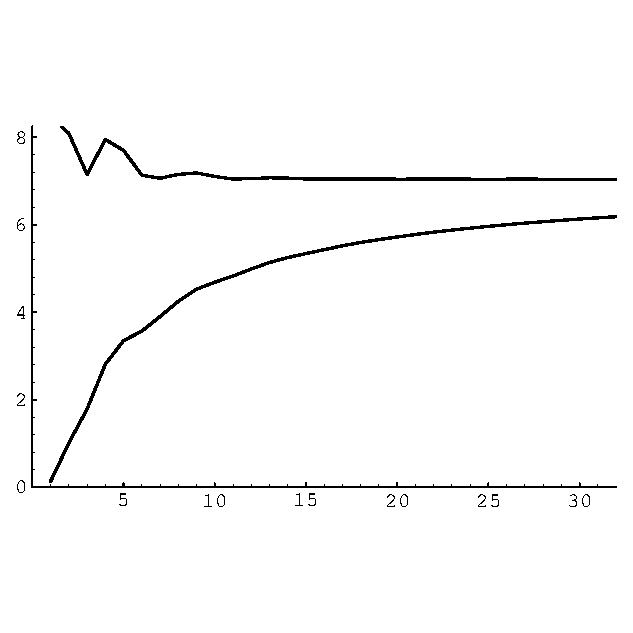
\includegraphics[width=3.25in]{graeffeb}
\end{center}
\caption{Upper and lower bounds on $M(P)$\label{Graeffe:Bound:Fig}}
\end{figure}

The lower bound of \propref{Graeffe:Bound:Prop} is not particularly
sharp, although the upper bound can be made quite sharp by increasing the
size of $k$.  

To illustrate this technique consider the following polynomial
suggested by \cite{Cerlienco1987-vl}
\[
P(X)  = X^6 + X^5 + 6X^4 - 5X^3 + 3X^2 + 2,
\]
which has zeroes
\[
-0.9015 \pm 2.4962 i, \quad0.6745 \pm 0.5646i, \quad
-0.2730 \pm 0.5408i.
\]
Only the first two zeroes are outside the unit circle and their
product is $7.0436280 = M(P)$.  \figref{Graeffe:Bound:Fig} shows the
upper and lower bounds on $M(P)$ based on $P_k$ as $k$ ranges from $1$
to $32$.  For $k = 11$ we already get the quite good upper bound of
$7.0470$, while the lower bound is $4.8284$.  For $k = 2048$, the
lower bound rises to $7.02934$, but computationally this is quite
expensive, due to the size of the coefficients of $P_m(X)$.

\section{Weighted Coefficient Bounds}
\label{Weighted:Bounds:Sec}


The relationship between $|p_i|$ and $M(P)$ given in
\eqnref{CoefZ:Bound:Eq} can be used to derive a bound on the
individual coefficients of divisors of a polynomial, as noted by
Mignotte \cite{Mignotte1974-oa}.  

\begin{proposition}[Mignotte]\label{Mignotte:Bound:Prop}
Let $Q(X) = q_0 X^{r} + q_{1} X^{r-1} + \cdots + q_{r}$ be a
polynomial over $\C$ that divides $P(X)$.  Then
\[
\left| q_{i} \right| \le \binom{r}{i} \left\|P\right\|.
\]
\end{proposition}
\begin{proof}
By \eqnref{CoefZ:Bound:Eq} we have,
\[
|q_i| \le \binom{r}{i} M(Q).
\]
Since every zero of $Q$ is a zero of $P$, we have $M(Q) \le M(P)$, and
by \propref{Landau:Zeroes:Prop}, $M(P) \le \|P\|$, which gives the
proposition. 
\end{proof}

This proposition indicates that the coefficients closer to the middle
of $Q(X)$ can be substantially larger than coefficients near the
leading and trailing terms.  Recently, this observation was made
substantially more precise by using the {\em weighted $L_2$ norm}.

Comparing the definition of the $[\cdot]_2$ norm \eqnref{PB:Beauzamy:Eq} 
with the lower inequality in \eqnref{CoefZ:Bound:Eq} we see that
\[
\sum_{0\le i \le d} \binom{d}{i}^{-1} |p_i|^2 \le
\sum_{0\le i \le d} \binom{d}{i} M^2(P).
\]
So, $[P]_2 \le 2^{d/2} M(P)$.  Applying the inequality to $M(P_1 P_2) = 
M(P_1) M(P_2)$, where $\deg P_1 + \deg P_2 = d$ gives:
\[
2^{d/2} \sqrt{d+1} |P_1 P_2| \ge [P_1]_2 \, [P_2]_2.
\]
More sophisticated techniques \cite{Beauzamy1990-yo} can be used to prove the 
following proposition.

\begin{proposition}
Let $f$ and $g$ be polynomials in one variable of degree $m$ and $n$
respectively.  Then
\[
[fg]_2 \ge \sqrt{\frac{m! \, n!}{(m+n)!}} [f]_2 \, [g]_2,
\]
and this result is best possible.
\end{proposition}

The following proposition \cite{Beauzamy1992-ts} is an analogue of 
\propref{Mignotte:Bound:Prop}, but uses the $[\cdot]_2$ norm. 

\begin{proposition} 
Let $P(X)$ be a univariate polynomial in $X$ over $\Z$, with
non-vanishing constant term.  Let $Q(X)$ be a divisor of $P(X)$, also
with rational integer coefficients.  Denote $\deg P$ by $d$, and $m =
\deg Q$.  Then each coefficient $q_i$ of
$Q(X)$ satisfies
\[
|q_i| \le \sqrt{\frac{1}{2} \binom{m}{i} \binom{d}{m}} [P]_2
   \le \sqrt{\frac{n!}{2(d-m)!\, (m-i)!\, i!}} [P]_2.
\]
Furthermore, 
\[
|Q| \le \frac{3^{3/4}}{2\sqrt{\pi}}\, \frac{3^{d/2}}{\sqrt{d}} [P]_2.
\]
\end{proposition}


\section{Size of a Polynomial's Zeroes}
\label{PB:RootSize:Sec}

The following inequality is due to {\Cauchy}
\cite{Cauchy1829-wp}.\Marginpar{Need intro}

\begin{proposition}[Cauchy]
\label{Cauchy:Zero:Bound:Prop}
Let $P(X) = X^{d} + p_{1} X^{d-1} + \cdots + p_{d}$ be a non-constant,
monic polynomial with coefficients in $\C$.  Then each root of $P(X)$,
$\alpha$, satisfies the inequality
\begin{equation}
\label{Cauchy:Zero:Ineq:Eq}
\left|\alpha\right| < 1 + \max \{|p_{1}|, \ldots, |p_{n}|\} 
  = 1 + \left| P \right|.
\end{equation}
\end{proposition}

\begin{proof}
Assume $|\alpha|$ is greater than $1$, otherwise the proposition is obvious.
By taking the absolute value of 
\[
\alpha^d = -(p_{1} \alpha^{d-1} + \cdots + p_{n}),
\]
we have
\[
\left| \alpha \right|^{d} = \left| p_{1} \alpha^{d-1} + \cdots + p_{n} \right|
 \le \left| \alpha^{d-1} + \cdots + 1 \right| |P| 
 \le \frac{|\alpha|^{d}}{|\alpha| - 1} |P|.
\]
Since $|\alpha| > 1$, we can multiply by $|\alpha| - 1$ which gives 
$|\alpha| \le 1 + |P|$. 
\end{proof}

In \propref{Cauchy:Zero:Bound:Prop} we assumed that $P(X)$ is monic.  If this is not the case, we
can monicize the polynomial and apply \propref{Cauchy:Zero:Bound:Prop}.  In
particular, let 
\[
P(X) = p_{0} X^{d} + \cdots + p_{d},
\]
and let $\alpha$ be a zero of $P(X)$.  Applying the proposition to
\[
X^{d} + \frac{p_{1}}{p_{0}}X^{d-1} + \cdots + \frac{p_{d}}{p_{0}}
\]
gives
\[
\begin{aligned}
|\alpha| & 
   \le 1 + \max\{ \frac{p_{1}}{p_{0}}, \ldots, \frac{p_{d}}{p_{0}} \},\\
 & \le \frac{\left|p_{0}\right| + 
               \max \{\left|p_{1}\right|, \ldots, \left|p_{d}\right|
\}}{\left|p_{0}\right|}.
\end{aligned}
\]
Applying \propref{Cauchy:Zero:Bound:Prop} to the monic polynomial of
$1/\alpha$:
\[
X^{d} + \frac{p_{d-1}}{p_{d}} X^{d-1} + \cdots + \frac{p_{0}}{p_{d}}
\]
gives
\[
|\alpha| \ge \ \frac{\left|p_{d}\right|}{\left|p_{d}\right| + 
   \max\{ \left|p_{0}\right|, \ldots, \left|p_{d-1}\right|\}}.
\]
Putting these two results together we have for each zero of $P(X)$,
\[
\frac{\left|p_{0}\right| + 
               \max \{\left|p_{1}\right|, \ldots, \left|p_{d}\right|
\}}{\left|p_{0}\right|}
\ge
|\alpha| \ge \ \frac{\left|p_{d}\right|}{\left|p_{d}\right| + 
   \max\{ \left|p_{0}\right|, \ldots, \left|p_{d-1}\right|\}}.
\]

\section{Discriminants and Zero Separation}
\label{PB:RootSeparate:Sec}

This section obtains bounds on the minimum difference between zeroes of a
polynomial $P(X)$.  One of the most useful expressions involving the
difference of zeroes of $P(X)$ is the {\em discriminant} of $P$, which
is essentially the square of the product of differences of pairs of
zeroes of $P(X)$.  This quantity is quite useful in the study of
algebraic extensions.

\paragraph{Discriminants}

As usual, let $\alpha_1, \ldots, \alpha_d$ denote the zeroes of
$P(X)$.   Consider the \keyi{Vandermonde matrix}
\[
P_D = 
\left(\begin{array}{ccccc}
1 & \alpha_1 & \alpha_1^2 & \cdots & \alpha_1^{d-1} \\
1 & \alpha_2 & \alpha_2^2 & \cdots & \alpha_2^{d-1} \\
\vdots & & \vdots & \cdots & \vdots \\
1 & \alpha_d & \alpha_d^2 & \cdots & \alpha_d^{d-1} 
\end{array}\right),
\]
which is discussed in some detail in
\sectref{Vandermonde:Sec}.  Its determinant is equal to the product of
the difference of the zeroes of $P(X)$:
\[
\det P_D = \prod_{1\le i < j \le d} ( \alpha_i - \alpha_j).
\]
The {\em discriminant} of $P(X)$\index{discriminant!of a
polynomial} is defined to be
\addsymbol{$\protect\Dscr(P)$}{The discriminant of the polynomial $P$}
\begin{equation}\label{PB:Discriminant:Eq}
\Dscr(P) = p_0^{2d-2} \det|P_D|^2.
\end{equation}

The discriminant of a polynomial can be computed using
resultants.  We write $P(X)$ as
\[
P(X) = p_0 (X - \alpha_1) (X - \alpha_2) \cdots (X - \alpha_d).
\]
Its derivative is
\[
P'(X) = p_0(X - \alpha_2) \cdots (X - \alpha_d) + \cdots + p_0(X - \alpha_1) \cdots (X -
\alpha_{d-1}).
\]
Evaluating at $\alpha_i$ we have
\[
P'(\alpha_i) = p_0(\alpha_i - \alpha_1) \cdots \widehat{(\alpha_i -
\alpha_i)} \cdots (\alpha_i - \alpha_d),
\]
where the circumflex indicates a term in the product that is omitted.
Taking the product over all zeroes of $P(X)$ gives
\[
\begin{aligned}
P'(\alpha_1) \cdots P'(\alpha_d) 
  & \displaystyle
    = (-1)^{d(d-1)/2} p_0^d \prod_{1\le i< j \le n}(\alpha_i - \alpha_j)^2,\\
  & \displaystyle
    = (-1)^{d(d-1)/2} p_0^{2-d} \Dscr(P).
\end{aligned}
\]
By the definition of the resultant \eqnref{Resultant:Def:Eq} 
(page \pageref{Resultant:Def:Eq})
\[
\res_X (P(X), P'(X)) = p_0^{d-1}P'(\alpha_1) \cdots
P'(\alpha_d),
\]
since either $d$ or $d-1$ is even.  Combining these two equations gives
\[
\Dscr(P) = (-1)^{d(d-1)/2} \frac{\res_X (P(X), P'(X))}{p_0}.
\]

This formula allows us to compute the discriminant of specific
polynomials quite readily.  In particular,
\[
\begin{aligned}
\Dscr(aX^2 + bX + c) & = b^2 - 4ac, \\
\Dscr(X^3 + bX + c)  & = -(27 c^2 + 4b^3).
\end{aligned}
\]
For binomial polynomials we have,
\[
\begin{aligned}
\Dscr(X^n +a) &= (-1)^{n(n-1)/2} \res_X(X^n + a, n X^{n-1}), \\
 & = (-1)^{n(n-1)/2} \res_X(X^n + a, n) \res_X(X^n + a, X)^{n-1}, \\
 & = (-1)^{n(n-1)/2} n^n a^{n-1},
\end{aligned}
\]
where we have used \longpropref{Resultant:Properties:Prop}.

For trinomials the computation is a bit more difficult, but we do have
the following result of {\Swan} \cite{Swan1962-lf}.

\begin{proposition}[Swan]
Let $m$ and $n$ be positive integers with {\sc gcd} $d$ and cofactors
$M$ and $N$ respectively.  Then
\[
\begin{aligned}
\Dscr(X^m & + aX^n +b)\\
  & =
 (-1)^{m(m-1)/2} b^{n-1} (m^M b^{M - N} - (-1)^M (m - n)^{M - N} n^N a^M)^d.
\end{aligned}
\]
\end{proposition}
\begin{proof}
By the definition of the discriminant we have
\[
\Dscr(X^m + aX^n +b) 
    = (-1)^{m(m-1)/2} \res_X (X^m + aX^n + b, mX^{m-1} + anX^{n-1}).
\]
Since
\[
X^m + a X^n + b = \frac{X}{m} \cdot \left( mX^{m-1} + a n
X^{n-1}\right)
  + a \frac{m - n}{m} X^n + b,
\]
we have
\[
\begin{aligned}
\Dscr(X^m &+ aX^n +b) \\
  & = (-1)^{m(m-1)/2}  m^{m-n} \res_X (a \frac{m - n}{m} X^n + b, mX^{m-1} + anX^{n-1}).
\end{aligned}
\]
The resultant in this expression can be evaluated by factoring
\[
mX^{m-1} + a n X^{n-1} = X^{n-1} \times (m X^{m-n} + a n),
\]
and computing the two resultants:
\[
\res_X (a \frac{m - n}{m} X^n + b, X^{n-1}) = b^{n-1}
\]
and 
\[
\begin{aligned}
\res_X &(a \frac{m - n}{m} X^n + b, mX^{m-n} + an)\\
  &\qquad\qquad\qquad\qquad =
\left(b^{M-N} m^N - (-1)^N \left(a \frac{m-n}{m}\right)^{M-N} a^N
n^N\right)^d
\end{aligned}
\]
using \longpropref{Binomial:Result:Prop}.
When these results are multiplied and expanded we get the proposition.
\end{proof}

\medskip
Using \longpropref{Resultant:Bound:Prop} we can bound $|\Dscr(P)|$ as
\begin{equation}\label{PB:DiscrmBound1:Eq}
|\Dscr(P)| \le (\deg P + \deg P')! \,|P|^{d-1} |P'|^d \le (2d-1)! \,d^d\,
|P|^{2d-1}.
\end{equation}


This bound can be sharpened by applying the \key{Hadamard inequality}
(\longpropref{Hadamard:Ineq:Prop}) to $P_D$.  First, let $\alpha_i$ be a 
zero of $P(X)$ with absolute value less than $1$.  For each row
of $P_D$, we have
\[
\|\langle 1, \alpha_i, \ldots \alpha_i^{d-1} \rangle\|_2
\le \sqrt{1^2 + 1^2 + \cdots + 1^2} \le \sqrt{d}.
\]

Now, assume the zeroes of $P(X)$ satisfy
\[
|\alpha_1| \ge |\alpha_2| \ge \cdots \ge |\alpha_m| \ge 1 \ge |\alpha_{m+1}|
\ge \cdots \ge |\alpha_d|.
\]
So, the first $m$ zeroes of $P(X)$ lie outside the unit disk.
Dividing the first row by $\alpha_1^{d-1}$, the second row by
$\alpha_2^{d-1}$ and so on, we have
\[
Q_D = \frac{P_d}{(\alpha_1 \cdots \alpha_m)^{d-1}} =
\left(\begin{array}{ccccccc}
\alpha_1^{1-d} & \alpha_1^{2-d} & \alpha_1^{3-d} & \cdots & 1 \\
\vdots & & \vdots & \cdots & \vdots \\
\alpha_m^{1-d} & \alpha_m^{2-d} & \alpha_m^{3-d} & \cdots & 1 \\
1 & \alpha_{m+1} & \alpha_{m+1}^2 & \cdots & \alpha_{m+1}^{d-1} \\
\vdots & & \vdots & \cdots & \vdots \\
1 & \alpha_d & \alpha_d^2 & \cdots & \alpha_d^{d-1} 
\end{array}\right),
\]
where each element of $Q_D$ has absolute value less than $1$.  By
Hadamard's inequality, $\det|Q_D|$ can be bounded by $d^{d/2}$.
Thus,
\[
\det|P|= (\alpha_1 \cdots \alpha_m)^{d-1} \det|Q_D| \le 
\frac{M(P)^{d-1}}{p_0^{d-1}} d^{d/2},
\]
in general.  This immediately gives the following upper bound for the
discriminant. 

\begin{proposition}
If $P(X)$ is a univariate polynomial over $\C$ of degree $d$ and
leading coefficient $p_0$ then the absolute value of the discriminant
of $P(X)$ is bounded by
\[
|\Dscr(P)| \le d^d M(P)^{2(d-1)} \le d^d \|P\|^{2(d-1)}.
\]
\end{proposition}

The last inequality follows from \propref{Landau:Zeroes:Prop}.  Lower
bounds for the discriminant are much more subtle.  We quote the
following results of {\Odlyzko} in this regard \cite{Odlyzko1975-do,Odlyzko1977-rt}:

\begin{proposition}
Let $P(X)$ be a univariate, square free polynomial over $\Z$ of degree
$d$.  Denote the number of real zeroes of $P(X)$ by $r_1$ and the
number of complex zeroes by $2r_2$.  Then
\[
\begin{aligned}
|\Dscr(P)| & \ge (60.1)^{r_1} (22.2)^{2r_2} e^{-254}, \\
|\Dscr(P)| & \ge (58.6)^{r_1} (21.8)^{2r_2} e^{-70}. \\
\end{aligned}
\]
Assuming the generalized Riemann hypothesis
\[
|\Dscr(P)| \ge (188.3)^{r_1} (41.6)^{2r_2} e^{-3.7\times10^8}.
\]
\end{proposition}


\paragraph{Zero Separation}

In order to numerically determine the zeroes of $P(X)$, a univariate
polynomial of degree greater than $1$, it is important to know when
two zeroes are identical.  Since we cannot have exact finite numerical
representations of the zeroes of $P(X)$, we need a lower bound on how
close two distinct zeroes of a $P(X)$ can be.  We define the {\em zero
  separation}\index{zero separation} of $P$ to be
\[
\Delta(P) = \min_{i \not= j} \left| \alpha_{i} - \alpha_{j} \right|.
\]
\addsymbol{$\Delta(P)$}{minimum zero separation of two distinct zeroes
of the univariate polynomial $P$}

Assume that $|\alpha_i - \alpha_j|$ is the difference of roots of
$P(X)$, $i < j$.  We will use a slight variation of the techniques
used for discriminants to get an upper bound on $\det|P_D/(\alpha_i -
\alpha_j)|$.  This immediately yields a lower bound on $\Delta(P)$. 

Start with $P_D$ and subtract the $j$-th row from the $i$-th row,
\[
\left(\begin{array}{ccccccc}
1 & \alpha_1 & \alpha_1^2 & \cdots & \alpha_1^{d-1} \\
\vdots & & \vdots & \cdots & \vdots \\
0 & \alpha_i - \alpha_j & \alpha_i^2 - \alpha_j^2 & \cdots &
\alpha_i^{d-1} - \alpha_j^{d-1} \\
\vdots & & \vdots & \cdots & \vdots \\
1 & \alpha_d & \alpha_d^2 & \cdots & \alpha_d^{d-1} 
\end{array}\right).
\]
$\alpha_i - \alpha_j$ divides the $i-th$ row of this matrix so
\[
\frac{\det|P_D|}{\alpha_i - \alpha_j} = 
\left(\begin{array}{ccccccc}
1 & \alpha_1 & \alpha_1^2 & \cdots & \alpha_1^{d-1} \\
\vdots & & \vdots & \cdots & \vdots \\
0 & 1 & q_2 & \cdots & q_{d-1} \\
\vdots & & \vdots & \cdots & \vdots \\
1 & \alpha_d & \alpha_d^2 & \cdots & \alpha_d^{d-1} 
\end{array}\right),
\]
where 
\[
q_{\ell} = \alpha_i^{\ell-1} + \alpha_i^{\ell -2} \alpha_j + \cdots +
\alpha_j^{\ell-1}.
\]
We now divide the first $m$ rows by $\alpha_{\ell}^{d-1}$ as before.
The elements of all but the $i$-th row have absolute value no
greater than $1$.  The absolute values of the elements of the $i$-th
are bounded by $0, 1, 2, \ldots, {d-1}$ respectively, since
$|\alpha_i| > |\alpha_j|$.  

Applying Hadamard's inequality gives
\[
\frac{\det|P_D|}{(\alpha_i - \alpha_j) (\alpha_1 \ldots
\alpha_m)^{d-1}} 
\le d^{(d-1)/2}\sqrt{0^2 + 1^2 + \cdots + (d-1)^2}.
\]
The sum of squares inside the square root is easily bounded:
\[
0^2 + 1^2 + \cdots + (d-1)^2 = \frac{m(m-1)(2m-1)}{6} \le
\frac{m^3}{3}.
\]
Thus,
\[
\frac{p_0^{d-1} \det|P_D| \sqrt{3}}{M(P)^{d-1} d^{(d+2)/2}} 
   < |\alpha_i - \alpha_j|.
\]
Applying \eqnref{PB:Discriminant:Eq} gives {\Mahler}'s bound on the separation 
of the roots of $P(X)$ \cite{Mahler1964-vy}.

\begin{proposition}[{\Mahler}]
Let $p(x)$ be a square free polynomial of degree $d$ with discriminant $D$.
Then
\[
\Delta(p) > \sqrt{\frac{3 |D|}{d^{d+2}}} M(p)^{1-d}
\]
\end{proposition}

Using \propref{Landau:Zeroes:Prop} we have
\[
\Delta(p) > \sqrt{\frac{3 |D|}{d^{d+2}}} \|p\|^{1-d}.
\]

\section*{Notes}

\small

\notesectref{PB:Heights:Sec} Emma {\LehmerE} \cite{Lehmer1936-dj} surveyed
the early work on the size the coefficients in cyclotomic
polynomials. {\BatemanPT} gave an upper bound on the size of the
coefficients of a cyclotomic polynomial.  They are bounded above by
\[
\log A_n <  \frac{1}{2} d(n) \log n  
\le \frac{1}{2} \frac{(\log 2) (\log n)^2}{\log \log n},
\]
where $A_n$ is the absolute value of the largest coefficient in the
$n$-th cyclotomic polynomial.  Here we have used the bound
\eqnref{DivisorUBound:Eq} in the final inequality.  {\Vaughn}
\cite{Vaughan1974-vf} gave explicit lower bound,
\[
\log A_n > \exp \left( \frac{(\log 2) (\log n)}{\log \log n} \right),
\]
which implies both results are best possible.
{\Apostol} \cite{Apostol1975-js} contains a good bibliography of more
recent results.

\notesectref{Uniform:Bounds:Sec}  A nice proof of
\propref{Jensen:Formula:Prop} is contained in problems 120 and 175,
part III of P\'olya and Szeg\"o \cite{Polya1978-hx}.
{\Gelfond}'s proof of \propref{Factor:CBound:Prop}
\cite{Gelfond1960-ev} (pages 135--139) uses only elementary
techniques but it is quite a bit more lengthy than the one provided
here.

Mignotte \cite{Mignotte1992-sr} gives a bound similar to
\propref{Landau:Zeroes:Prop} but which uses a product of the $n$
largest roots, not all the roots. 

Alternative, more efficient approaches to the Graeffe method of
computing $M(P)$ are discussed in \cite{Cerlienco1987-vl}.  One interesting
observation that can be made from \figref{Graeffe:Bound:Fig} is that
the $\|P_k\|^{1/k}$ tends to be an especially good bound on $M(P)$
when $k$ is a prime number.  Can this statement be made more precise
and generalized?\Marginpar{Also checkout \cite{Boyd93a,Boyd93b,Mignotte94}.}

\notesectref{PB:RootSeparate:Sec} The presentation here follows that
of {\Mahler}'s original paper \cite{Mahler1964-vy}.
{\Mahler}'s proposition gives a lower bound on the separation of any pair 
of zeroes of a polynomial.  If a bound is only needed for a separation of 
real roots, then a bound of {\Rump} can be used that is a bit sharper 
\cite{Rump1979-dt}:
\[
\Delta_{real}(P) > \sqrt{\frac{8}{d^{d+2}}} \, \left(\frac{1}{1+|P|^d}\right).
\] 
\normalsize
